\documentclass[UKenglish]{ifimaster}
\usepackage[utf8]{inputenc}
\usepackage[T1]{fontenc, url}
\usepackage{graphicx,babel,csquotes,textcomp,ifimasterforside,varioref,float}
\usepackage[backend=biber,style=numeric-comp,sorting=nyt,maxbibnames=20,maxcitenames=20]{biblatex}
\urlstyle{sf}
\graphicspath{{images/}}
\addbibresource{macros.bib}
\addbibresource{references.bib}
\title{Ranklust}
\subtitle{A bioinformatics solution to identify network biomarkers in cancer}
\author{Henning Lund-Hanssen}

\begin{document}
\ififorside{}
\frontmatter{}
\maketitle{}

\chapter*{Abstract}
This is where the abstract goes...

\tableofcontents{}
\listoffigures{}
\listoftables{}

\mainmatter{}

\part{Introduction}
To this day we still struggle with cancer. Even with all our modern equipment and knowledge we have still not been able
to tame this horrible disease. 

% Cite "modeling genomic regulatiry networks with big data"
And even if we have all of this new equipment, most molecular biologists does not have the experience nor the competence
to use the newfound equipment or interpret the results. This is where bioinformaticians come in. 

% Rewrite this and use sources! It should explain incidence, pure and simple.
Incidence is the increase in the rate of new occurrences. So if we were to analyze the amount of new HIV incidents over
10 years and we start with 20 incidents, then after 5 years we get 20 new incidents and then after 10 years, we get 30
new incidents. We now have a total of 75 new incidents since the start (25 + 20 + 30).  Because we do not know when the
20 first incidents in the first 5 years happened, we assume they happened after 2,5 years (halfway to 5 years). So we
will get 20 * 2,5 and end up with 50 possible new cases. Do the same with the next 5 years and the next 30 new
occurrences! The only exception to the previous calculation is that we know they happened somewhere between 5 and 10
years, so we go halfway, to 7,5 ((5+10)/2 = 7,5) and do the same calculation: 7,5 * 30 = 225. Then combine them, 225 +
50 = 275. We ignore the first change, since they are what we started with. Let us also define the sample size of the
population to be 225. We then know that 150 people did not get HIV during the 10-year period. So if we were to add these
150 people over the 10 years that did not receive HIV, we get 150 * 10 = 1500. We add the increase of HIV, which is 275
and get 275 + 1500 = 1775. 

My thesis is about making a tool, named Ranklust, which gives cancer researchers an easier way of identifying network
biomarkers in cancer. 

\chapter{Motivation}
Biomarkers are at the centre of this thesis. They are what Ranklust should be able to detect and rank in order to
identify network biomarkers, and not just single molecules of them. A biomarker is a "biological measure of a biological
state" \cite{biomarker1}. It can be represented by the levels of a specific protein in our blood, a specific gene, or a
combination the two.

Biomarkers can be used for different purposes. They can be used to measure the effect of cancer drug treatment. That the
drug does what it is supposed to do. It can be used to predict disease development or the current stage of the disease.
Here is a list of what biomarkers currently are being used for:
\\\\
\textbf{Usages for biomarkers:} \cite{beyondpsa}
\begin{itemize}
    \item Disease disposition
        \begin{itemize}
            \item What is a patient's risk of developing cancer in the future?
        \end{itemize}
    \item Screening
        \begin{itemize}
            \item Does earlier detection of patients with cancer decrease mortality?
        \end{itemize}
    \item Diagnostic
        \begin{itemize}
            \item Who has cancer? What is the grade of the cancer?
        \end{itemize}
    \item Prognostic
        \begin{itemize}
            \item What clinical outcome is most likely if therapy is not administered?
        \end{itemize}
    \item Predictive
        \begin{itemize}
            \item Which therapy is most appropriate?
        \end{itemize}
    \item Monitoring
        \begin{itemize}
            \item Was therapy effective? Did the patient's disease recur?
        \end{itemize}
    \item Pharmacogenomic
        \begin{itemize}
            \item What is the risk for adverse reaction to the prescribed therapeutic dose?
        \end{itemize}
\end{itemize}
\textbf{Characteristics for a good biomarker:}
\begin{itemize}
    \item Safe and easy to measure
    \item Cost efficient to follow up
    \item Modifiable with treatment
    \item Consistent across gender and ethnic groups
\end{itemize}

%% New part in Motivation - should it stay or be rewritten?
The National Institues of Health Biomarkers Definitions Working Group has defined biomarkers as "a characteristic that
is objectively measured and evaluated as an indicator of normal biological processes, pathogenic process, or
pharmacologic responses to a therapeutic intervention.". The World Health Organization (WHO) has created a guideline for
defining biomarkers: "almost any measurement reflecting an interaction between a biological system and a potential
hazard, which may be chemical, physical or biological. The measured response may be functional and physiological,
biochemical at the cellular level, or a molecular interaction". So a biomarker kan be anything from the pulse of the
heart or blood pressure. In this thesis, I will see if we can get better and more information from ranking gene and
protein clusters based on biomarker information. The result could in the best case be a new biomarker in itself, and can
be a step in the direction of hierarchical biomarkers (biomarkers creating new biomarkers).


Biomarkers versus Clinical Endpoints Some of the important characteristics of biomarkers is that they are objective and
quantifiable as biological processes. They are used as a state indicator of the biological object that is under
scrutiny. When the biological object is a human being screned for cancer, biomarkers may help.

Biomarkers can be an indicator of how far cancer has progressed in the human body. But the human subject may feel no
difference at all. It can also be the opposite, that the human subject feels huge differences during several weeks that
the cancer might have developed at a grand scale, but the biomarkers show no objective change. This proves that the
human subject's experience and sence of state that it is in does not necessarily have to correlate.

Clinical endpoints is the opposite. They describe how the subjects feel or describe how they function. It is not as
objective as biomarkers and it demands more resources to gather the information, as the subjects has to be interviewed
in some form, rather than interpreting pure data. But one thing has to be noted; patients does not seek treatment for
cancer due to their biomarkers being "off the charts". They seek treatment because they \textit{feel} that they do not
feel ok or do not function sufficiently. So biomarkers are not by any means far superior to clinical endpoints in all
aspects.

Biomarkers can also be ruled out as a reliable predictor when population differences are too big. As with clinical
endpoints, people describe their feelings differently and might hold information back. As pointed out before, people's
feelings are subjective, and different ways of interpreting their own body's state might skew statistical results with
erronous feedback. Erronous feedback in this case can be examplified as two persons who are at the exact same state of
cancer, with the same prerequisites, but they report how they feel differently. One person might be ignoring certain
pains or lose hair aftern radiation treatment, but not the other. This can be mitigated to some degree with careful and
accurate screening of patients admitted to treatment, but a totally unified group in terms of how they describe pain and
other attributes that are interesting might be seen as borderline impossible. We are afterall humans and very much
fallible.

%% CITE GLOBAL CANCER START ---
In 1990, cancer was the third leading cause of death. By 2013, it has taken second place and the amount of deaths
related to cancer is considered to be doubled by 2030. For men in particular, the highest incidents of cancer came from
prostate cancer, with a count of 1.4 million incidents. For women, breast cancer tops the statistics at 1.8 million
incidents. For both sexes, tracheal, bronchus and lung cancer tops the list at 1.6 *deaths*, not incidents.

The increasing number of cancer-related incidents is a big threat in countries that are not adequate equipped to deal
with complex and expensive cancer treatments.

With a stable population growth and age structure, we would have seen a 13\% decrease in incident cases between 1990 and
2013. Instead, incident cases has increased by 67\%

Incidence cases for women has risen slowly whereas for men, it has decreased.

Breast cancer is the most lethal cancer for women. Only 1\% of breast cancer cases occur in men. Between 1990 and 2013,
incidence cases of breast cancer has increased by 99\%. Taking into account a stable population and age structure, it
falls to about 26\%, which still is a significant increase in incidents.

Prostate cancer incident cases increased by 217\% in period 1990 to 2013.  Increased life expectancy is expected to
contribute somewhere between 20\% and 43\% to the increase in this occasion.

217\% on a global scale, 167\% in developed countries and 367\% in developing countries. Age alone cannot explain the
HUGE increase in developing countries.  But it may show a bigger need for prostate screening in low-/middle-income
countries.

Even though developed countries has 70\% higher ASIR, the ASDR is only 20\% higher in developed countries, showing that
the cancer is detected, patients in developed countries has a higher chance of survival (not very surprising...).

An example of a single molecule biomarker is the prostate specific antigen (PSA). This is a protein produced by the
prostate gland in male humans. The identification of cancer with PSA is simple, the higher the level of PSA, measured in
ng/mL (nanograms per milliliter), the higher is the chance of the patient having prostate cancer \cite{cancerfacts}.

Today PSA is used for both identifying and evaluating the current stage of prostate cancer. This biomarker can be found
by analyzing blood examples from patients, thus fulfilling some of the demands for a good biomarker, but not all of
them. It is easy to measure and easy to acquire, but not reliable enough to be used as the only marker to identify and
determine the stage or remission of prostate cancer. The low grade of reliability comes from the fact that even though
higher levels of PSA shows higher chance of having prostate cancer, prostate cancer is not the only reason to have
elevated levels of PSA \cite{cancerfacts}. Namely inflammation and enlargement of the prostate. Though, a man with both
of these cases may or may not develop prostate cancer.
%% CITE GLOBAL CANCER END ---

% Conclusion about PSA
So the conclusion for the PSA biomarker is that it is not reliable enough and are causing faulty treatment of prostate
cancer that may not even exist. Because even if a patient has prostate cancer, it may not be harmful, promoting the case
of not taking any action against it at all. So there is need for a new biomarker, or at least a better way to diagnose
and predict the right treatment.

\chapter{Next-generation sequencing}
Today, rapid analyzing of genes and proteins are made available through Next-Generation Sequencing (NGS)\cite{ngs1}.
% Find a better source for this!
Networks offers us an informatics, algorithmic, visual and mathematical tool to study this bigger picture. This project
will integrate the opportunity networks offer to discover new biomarkers in cancer.  Through acquiring more data, faster
than before, there now exists databases with much information that is easy to access. This makes room for building huge
networks of proteins and genes, allowing for more extensively and thorough assays to be done. For example, what if
something that is classified as a prostate cancer biomarker only is viable when proteins that has not been classified as
a biomarker, also is present? Together they could represent a more appropriate
\emph{network biomarker}.
The amount of data that can be analyzed also opens up for another more personalized approach to each cancer patient.
Finding patient-specific biomarkers could make a huge impact on the quality of treatment \cite{personalized}.
\chapter{Next generation of biomarkers}
The PSA biomarker is over 20 years old \cite{psa-age}. Through those years, it has been discovered other and better
biomarkers for prostate cancer than PSA. Among those, PCA3, which is detectable through urine samples from patients. It
also has the benefit of not being affected by the size of the prostate gland \cite{pca3-size}. But still the results
could be better. Therefore, it has been tried to combine these two biomarkers in order to see if it is beneficial to see
the results from each biomarker in light of each other \cite{beyondpsa}. The results from these tests is that they
complement each other to a level of significance that makes it compelling to analyze them both to diagnose prostate
cancer. It is important to point out that even if these biomarkers are not the best at indicating if a patient has
cancer or not, these biomarkers are good at indicating progression and recurrence of prostate cancer.

But all of this is based on single genes or proteins. What if we looked at whole networks as biomarkers?

\chapter{Networks as a tool in cancer research}
%Shit goes dooown \cite{networkmodels}.
%\begin{itemize}
%    \item Cells contain a vast array of molecular structures that come together to form complex, dynamic, and plastic
%        networks
%    \item For example, where in the molecular network of a tumor should we perturb with drug to reduce tumor
%        proliferation or metastasis
%    \item mTOR having poor results in clinical trials and even having subsequently increased cell proliferation
%    \item For example, if protein A induces expression of protein B, then we expect to see high leveles of protein B
%        whenever levels or specific molecular states of its activator A are high. The reverse of this logic is that
%        statistical correlation between protein states indicates a potential interaction between them
%    \item Although nonlinear relations frequently occur in biology, linear regression models are more robust, and thus
%        they often give better results, even when the underlying model is nonlinear
%    \item Networks are not fixed: The role of context and dynamics
%\end{itemize}
Viewing the cell as a network of proteins and genes presents us with several assumptions to make. Firstly, there is no
physical connection between the proteins and genes, which represents the nodes in the network. So a way of defining
edges between nodes has to be established. It exists several ways of doing this, but there has yet to be discovered a
silver bullet of defining the edges. % cite?

Bayesian probability networks are one way of defining edges \cite{bayesiannetworks}. It is based on the probability that
if a node A exists, then node B exists. That way it is possible to create networks based on the assumption that if node
A exists, then node B is 80\% likely to exist. Maybe node C and D have a 100\% chance of existing if node B exists.
These percentages represents how strong the edges between the nodes are, and makes it able to construct a directed
acyclic graph, DAG for short. It is important to note that a true bayesian network can not be achieved through random 
observations. Rather should some constant value(s) be introduced to be able to really measure the effect of the other
variables.

The way of defining edges in a network also determines what kind of information that is possible to get from it. The
different bio-databases has different ways of calculating edges. Should the database alone define the edges? If the
database supply weights in the edges and/or nodes, should it be used, changed or ignored? The final decision of how and
in what way the edges should be defined has yet to come. 

% Abstract 
They have studied 50 cancer types that have been cataloged by the International Cancer Genome Consortium (IGCC). They
found that only a few well-studied driver genes are frequently mutated, in contrast to many infrequently mutated genes
that may also contribute to tumor biology.

% Introduction
There is only a few altered genes that have a mutation frequency higher than 10\%, and a shitload of genes that have a
mutation frequency of 5\% and lower.  Prostate cancer is a type of cancer that has relatively few Single Nucleotide
Polymorphisms (SNPs) and Copy-Number Alterations (CNAs). This indicates that prostate cancer is probably driven by some
other type of somatic variation. The way driver genes are found is by identifying positive-selection signals.

%EXPLAIN positive-selection signals here!!!


%CONTINUE: 
With this approach the genes that are less frequently mutated, but are functionally important genes, will not be
detected by statistical analysis.  Another way detecting driver genes is by grouping the genetic alterations we can find
through knowledge about cellular mechanisms. This way will provide information about the affected oncogenic pathways.

% Pathways and networks
%% Difference between pathways and networks
Pathways are small networks of well studied processes where many areas are well documented. Networks on the other hand
are bigger and less explored, but when properly analyzed, it might provide new information unknown to pathway systems.

%% Pathways and networks vs. individual genes
Analyzing pathways and networks have an advantage over individual genes. They may reveal information that comes from
molecular events that covers multiple genes or pathways. Aggregating this data increases the chances of detecting driver
genes through statistical analysis (source 15). Also, information gathered through pathways and networks may be enriched
through genomic, transcriptomic and proteomic data and create a more unified view of the tumor biology.


\chapter{Network clustering: Toward network based biomarker discovery}
Networks is the pre-processing of single gene prioritization that is necessary in order to come to the next step,
clustering of the network. Clustering is about making a hierarchical view of a network to be able to look at the bigger
picture of the cell. The reason to group a network into clusters and rank them is that the edges we create represents
different connections. They can represent function, probability of existence, interactions or contents of the cell
\cite{siri}. The function of the cell is what Ranklust is after. There is several algorithms to create clusters, and all
need to be heavily researched in order to find the best suiting one. The major differences on how these algorithms work
is centered around how they handle vertices and edges. For example how the cluster is expanded, what density level it is
aiming for, how robust the algorithm is towards incomplete networks. It is feasible if the cluster-making algorithm is
easily, or even already implemented as an app in Cytoscape. ClusterMaker2 is such an app and will be considered
\cite{cm2}. But there is faster cluster-creating algorithms than those implemented in ClusterMaker2, namely the SPICi
\cite{spici} algorithm. So a possible solution for Ranklust could be to implement the SPICi algorithm into the
ClusterMaker2 app, in order to reuse most of the code that represents the GUI, single gene prioritization and network
creation. In addition to the cluster-creating algorithms, there is a need for cluster-ranking algorithms. They should be
ranked in the order of being a biomarker for cancer.

% Find a way to prove that, by severing the interaction bond between genes/proteines, you can stop cancer biomarkers
% from "communicating

The secretome of certain genes can be interpreted as biomarkers (source). CONTINUE HERE!

\chapter{Cytoscape: An implementation to rank clusters}
% Rename the Cytoscape section to Software/Architecture/Development
% General description of development
Cytoscape is the open-source software platform the Ranklust app will be developed on. Its main purpose is to visualize
molecular interaction networks and biological pathways.  It is easy to integrate \textbf{\textit{Apps}} and even combine 
multiple apps to solve new problems, given that the source code of the apps is available or that it exists an easy way of 
piping results from one app to another. 

The goal of Ranklust is to cluster the networks we get from single gene prioritization and rank them in order to 
identify network biomarkers. Apps taking care of making the networks already exists, but there still has to be made a 
decision about whether or not they could be modified in order to better support the clustering.

% Cytoscape
Cytoscape is based on the Java programming language, which is a little bit untraditional for a software platform used to
develop bioinformatics tools. % cite needed!!!
The reason to choose Java above Python, Perl or other popular programming languages is simply because I am more
versed in Java programming than any other language. Java is known for being this big bloated 
enterprise programming language, and Python as the fast and easy mockup tool to develop good programs fast. Python also
has big biological computation libraries like \emph{Biopython} \cite{biopython}, that makes it easy to build your own
standalone apps. Though when used in a bigger environment as Cytoscape, Java shines, having sturdy packaging and
modelling standards. The Cytoscape community is big, alive and has standards for how the architecture of apps should
look like. The community promotes this through the use of the \emph{OSGi} standard \cite{cytoscape-osgi}.

% OSGi and design patterns
Developing OSGi software should promote modularization \cite{modularization} % unreliable source?
of the code and increase the probability of the app being launched as an official Cytoscape app; in addition to provide
other developers with the possibility of reusing my modules in their own apps. Also, it seems like Java 9 is aimed
at making it easier to modularize apps along the lines of the OSGi standard, so it might be easier to refactor an
application in the future from Java 8 to Java 9 when the architecture already is in place. There exists several design 
patterns that could prove to be useful in the development of Ranklust. Another strategy to follow may not be a direct 
design pattern \cite{designpattern}, but more of a collection of them, is the clean code principles by Robert C. Martin
\cite{cleancode}. More thorough examination of these strategies will follow.
% find a better cleancode reference. Free edition of online book maybe?
% Or summary of clean code's abstract/introduction?

% Prototype section
Prototyping of different parts of the app will be done in Python and the Galaxy environment \cite{galaxy}. Python is an
easy language to prototype with, and Galaxy is an easy environment to test small scripts in. Galaxy also has great
logging of previous experiments combined with settings, so recreating simulations and comparing results is easy to do and
reliable. However, in my experience, Java comes up to par with Python in development speed once all of the boilerplate
code is written and a good deployment tool is used. Therefore the Cytoscape platform is used for the final deployment of
Ranklust.

% Maven section?? Other devtools? Cy3 Performance Reporter to measure the performance of SPICi inside clusterMaker2?

\chapter{Methods}

\chapter{Databases}
Using databases helps with several things. CONTINUE!!!

Which databases to use has to be considered. The reason to use databases is because they have information about how 
protein and genes form a network based on how they interact with each other. The initial database candidates in Ranklust 
are iRefIndex \cite{iri}, GeneMania \cite{gm} and STRING \cite{str}. These databases all have in common that it exists
Cytoscape apps made to use these databases. STRING however, does not have any repository available through the Cytoscape
app store, so interacting with the database through a new app in Cytoscape without making new plugins may be difficult.
On the other hand, both iRefIndex and GeneMania have their repositories easily available to the public together with
decent documentation. However, the difference between them is what they contain information about. iRefIndex contains
data about protein-protein interaction (PPI), while GeneMania contains data about genes.
% Check this next one out! Link from source!
Since proteins come from genes, GeneMania can also give us some information about proteins. Differences between the
two databases will be discussed in greater depth at a later stage.
The open-source plugins in Cytoscape to communicate with the databases are iRefScape \cite{iridb} for iRefIndex and 
GeneMANIA \cite{gmdb} for GeneMania.

% Neo4J Dump problem
A problem with the Neo4J database is the dump it creates. The dump creates a single Cypher (source: cypher) commit for
the whole database. This way, if anything goes wrong while importing the data, it will get rolled back. It hinders
faulty data and relationship between several parts of the data to be imported into the database. The problem with a
single commit to import the data is the required memory. My personal computer and the computers at University of Oslo
that I have access to does not have enough memory to import the database as a single commit in Cypher. Splitting up the
dump to several commits does not work without quirks. It conquers the memory problem, but the way the relationships
are created from the Neo4J dump requires the import process to be done in a single commit. A way to fix this is either
to not use Cypher queries as a way of importing the data, but instead use GraphML. Another way is to refactor the cypher
dump so that the creation of relationships does not need to be done in a single commit. I will use both ways, because
not being able to use the Cypher queries because of too little memory will most likely be a problem for several people
and not just me. Using GraphML is good for exporting data from CytoScape and from the database, but interaction between
the two of them while performing the algorithms is not feasible at the time. This last drawback is where Cypher queries
are good, because it exists plugins that aid in using data from the database directly in CytoScape. So initializing a
database for testing could easily be done with GraphML, and then use Cypher queries to perform the computations on the
data.

Creating a script to refactor the Cypher queries does not only help in regards of using the data with CytoScape, but
also for everyone using a Neo4J Cypher dump to create a database and does not have much memory. A problem that might
come up is performance. Because the current way of creating relationships use node labels in Neo4J and it takes only a
single line to create a relationship between two nodes. If I refactor the relationship-part of the Neo4J dump, it will
increase to a two instruction query. Firstly, two nodes has to be found based on their indexed node name, which will
relate to the protein/gene name. Secondly, I do the same thing that was done before the refactor, I create the
relationship between the two nodes. The difference between the old and the new way of creating the relationship is how
the nodes are found. The Neo4J dump creates temporary node variables prepended with an underscore and an integer ID.
These ID's only exist within the commit the nodes are created. So splitting creation and relationship-making leaves us
with worthless IDs that does not refer to any known node. That is when Neo4J tries to be smart and then creates new
nodes based on the underscore ID and then creates a relationship between them. The end result, two new nodes that only
contains the undescore IDs. So the refactored version aims at matching the underscore IDs in the relationship creation
to the node creation, and to replace them with the name of the nodes instead of the temporary underscore ID. But as
mentioned, matching the nodes with the name takes up more time and performance might be an issue. For comparison, with a
Cypher dump of 4500 lines, it takes about 20 seconds before the query engine gets a stack overflow (explain stack
overflow?). With GraphML, an XML file with 250000 lines takes under 1 second to import and it gets relationships right
without any form of refactoring.

\chapter{Clustering algorithms}


\part{Images testing...}
\begin{figure}[h]
    \caption{Cancers Ranked by Number of Incident Cases in Both Sexes, Globally, by Development Status, and in the 50
            Most Populous Countries, 2013}
    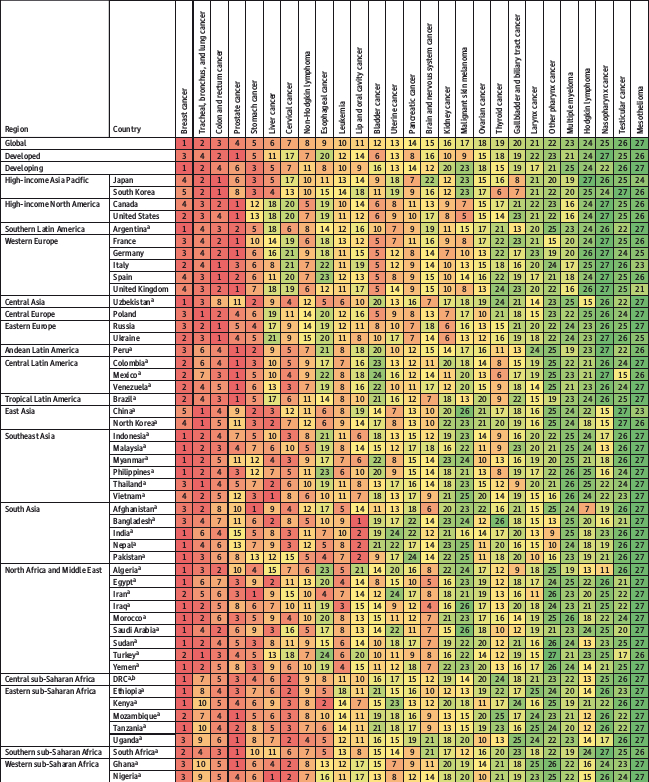
\includegraphics{cancer_incidents}
\end{figure}

\begin{figure}[h]
    \caption{Cancers Ranked by Number of Deaths in Both Sexes, Globally, by Development Status, and in the 50 Most
            Populous Countries, 2013}
    \includegraphics{cancer_deaths}
\end{figure}

\part{The project}
\part{CytoScape} % Make this a subsection in "The project" part
The structure of the code in CytoScape follows the already established structure in the ClusterMaker2 plugin. This is to
make it easy to maintain for the other contributors of ClusterMaker2. At the same time, the code is modularized enough
to make it easy to extract the code, in order to make a separate plugin. The motivation for having a separate plugin to
rank clusters in CytoScape gets bigger if ranking clusters provides useful information, in regards of discovering
cancer.

Adding new ranking algorithms should be easy both to implement and unit test. Where the algorithms should be placed and
how to connect it to the rest of the GUI in order to choose it, should be a no-brainer. Unit testing of the algorithms
should be possible without using the GUI. So all of the logic in the algorithms should be excluded from the GUI. If it
is not excluded from the GUI, testing the algorithms would require menu interaction and automatization of testing goes
out the window. Every test should be able to just run in the terminal without launching CytoScape. Mockup data % explain mockup data
should not be provided in source-files, but instead from files that can be read through the CytoScape API. % Why??

The "Factory" design pattern % reference
is used in a original way in ClusterMaker2, and for the ranking cluster algorithms it is done a little bit different.
The GUI will not be responsible for knowing every available algorithm, it will be the algorithm factory's. The GUI's way
of knowing which algorithms the user should be able to choose from, will be to ask the factory for a list of all of the
available algorithms. This is an example that shows by separating the amount of components that have knowledge about a
specific piece of information, it becomes easier adding new features. If the GUI also would have to construct a list by
itself about the available algorithms, in addition to the factory, we would end up making changes in two places instead
of just one. Twice the work for just one change - adding a new algorithm.

%%%%%%%%%%%%%%%%%%%%%%%%%%%%%%
%%%% IMPLEMENTATION START %%%%
%%%%%%%%%%%%%%%%%%%%%%%%%%%%%%

% Intro
The \textit{clusterMaker2} documentation for implementing new parts that is not directly connected with clustering
algorithms is non-existing (cite documentation!). So I will make a walkthrough of how to do it and how I did it.


% Preparations
The POM-file has to be updated because libraries connected to the pdf exporting functionality is outdated. Updating the
libraries, imports and the usage of these libraries in the source code is enough to make the whole project compile at
the mentioned date.

% Registering a service
In order to make it easy to implement new cluster ranking algorithms, a new task factory for the ranking of clusters is
required. It has to be registered as a service to make it visible to the GUI menu, aswell as maintain the \textit{OSGi}
standard of components added to the \textit{clusterMaker2} project. Also, creating a standalone plugin at a later stage will
be easier if Ranklust is properly compartmentalized.

Registering a new service listener is a way of keeping the Ranklust part out of clusterMaker2. Though, it is still
packaged within clusterMaker2's API, so that it does not become a mess, if extra functionality is to be implemented
while the plugin resides within clusterMaker2.

% GetNetworkClusterTask
ClusterMaker2 already has some REST (insert: reference to REST services + explanation). It is used in Ranklust as a way
of getting the clustering results without changin the previous code. Though, there is a flaw in the REST service. If the
clustering algorithm you want the results from is not the last clustering algorithm that was run on the network, it will
not be able to get the results. For now, this will stay as it is, but it should be brought up for discussion to rather
look up the table of the nodes instead of the table of the network, in order to get the clustering results. This is
because the table of the network can only hold a single value for clustering algorithms, which will either be nothing,
or the last algorithm run on the network. The drawbacks of looking up the table of nodes instead is the time it
consumes. But the time consumed to get all of the nodes with a specific clustering result attribute will take a shorter
time than to rerun the algorithm you want to have the results from. A third solution can be to just ignore the algorithm
used to cluster the network, as it should not have anything to say for the ranking of the clusters. This may end up
being the final solution, as it easily can be viewed as a more "sane" (formulate this in a different way). This option
requires a new REST function to be added to clusterMaker2. As a whole, it is highly possible that this new REST
functionality should replace the existing one. The argument to replace the already existing algorithm is that REST
functionality should hide state and implementation from the services using the REST service to get data. The way it is
now, this is not true and it should be changed anyway.

% Tables vs pure OO
One thing in particular that deserves to be mentioned is the way networks are handled. The \textit{CyNode} objects
themselves does not contain much. This is because all of the information is saved in the form of plain cells in a
spreadsheet. This may at first seem like a way to make it easy to show information to the user, but it is also a way of
working more efficient with network data (insert: reference to working with tables on networks is efficient). Creating
objects with attributes for each node in a huge network will increase the amount of overhead by a pretty noticable
amount. Working with all of the information in the way of a spreadsheet with rows and columns includes a decrease in
overhead. A new node is a new row, so in relation to build the network structure, it is not a difference to speak of.
The difference comes in when the nodes have several attributes. 

In a table or spreadsheet, attributes can be represented as a single column and be created once for the whole network,
instead of once for each node object created. This assumes that getting the objects out of the table is possible by
either indexing on a number for arrays, or a unique string for map structures. The result is both a lookup, insertion
and deletion time of O(1) (insert: reference to Big-O notation).  These times is as law as the Big-O notation goes in
terms of speed related to the size of a collection inside a data structure. So both the creation of objects goes down,
and the retrieval of attribute information is as low as it is possible to get, when we choose to represent the time by
Big-O notation. The only drawback with this implementation is that there is no current type of wrapper around the row
and column system. So the retrieval of information is not done the most intuitive way. But this is the way CytoScape
works as a whole, so changing the way this works is either done through changing the CytoScape source code, or
implementing a wrapper as a standalone function inside clusterMaker2 or as a standalone plugin.

% Single value ranklust
A simple, but effective way of ranking clusters, is just to add together the biomarkers values and sum them up in each
respective cluster. This will tell us which cluster will have the most cancerous genes and proteines. It is not very
advanced, but an analysis show how effective it is. An alternative is also to add scaling to the values. Should clusters
with a large amount of biomarkers receive a bonus because of the sheer amount? Should values alone be scaled exponential
in order to magnify the differences between more and lesser cancerous biomarkers? This will be tested in the final
stages of single value ranking in Ranklust. But as a beginning, the results will come from a pure additive algorithm.
The more advanced ones will be implemented only if the additive algorithm show promising results.

% Multivalue Ranklust
Multivalue ranking of clusters creates a larger context. More data can help making more fine tuned results and get the
validation of ranking clusters to find biomakers, hit the significance ceiling of 95\% certainity. % Fix this sentence!
The question here is how should several values be combined in order to create a single value score to rank the clusters
by? The best way should be to list every attribute to the user, and present them with options as to how the values
should be scaled. An extra option could be how to scale the values in relation each other. The first way is the simplest
way to implement so it will be tested first. And as with the single value ranking, if the first scaling of each
individual value shows promising results for multivalue ranking, the values in relation to each other will be
considered as a way of producing more accurate results.

%%%%%%%%%%%%%%%%%%%%%%%%%%%%%%
%%%% IMPLEMENTATION END %%%%%%
%%%%%%%%%%%%%%%%%%%%%%%%%%%%%%

\part{Procedure}
The secretome values of genes can be expressed by a single integer value, though, for compatibility reasons Ranklust
will require double values. The clustered network can be constructed with an AP, short for Affinity Propagation,
clustering algorithm (source AP). Affinity propagation clustering concentrates on the nodes in the network that are
binding the rest of them together. Using affinity propagation for clustering will produce results that represent a
grouping of nodes that are coupled by seemingly unimportant nodes to most clustering algorithms. But the AP algorithm is
good at expressing nodes that are not highly connected to many nodes, but rather the nodes that are binding other highly
connected nodes together. This results in bigger clusters that can be a target for methods that cure cancer by severing
the interaction between biomarker genes.

It is also discussed how AP performs versus Markov clustering (source, both markov algorithm and the "vs" paper). And
since Markov algorithm performs better on protein interaction, it will also be used to cluster the networks. An analysis
between the rankings that come from the Markov and AP clusterings will be performed, which hopefully will give concrete
results as to the pro's and con's of each algorithm. Some questions should be raised as the analysis is done. For
example, is both of the algorithms good, but have different uses, even if they are not directly involved with the
ranking done after the clustering? Are either AP or Markov useless for a particular type of ranking afterwards?

The information provided through the whole process from what type of nodes (protein or gene), interaction between the
nodes and what kind of biomarker we want to identify are all factors that will have a great impact on how all of this
should be combined. The order of operations on the network will also effect the result. For example, AP clustering may
create a few big clusters and many small ones. At this stage, the results will consist of the biggest clusters
constructed from AP clustering that has focus on pure connection between nodes and not their attributes. At this point,
the cluster ranking algorithm of Ranklust will be run in order to produce a picture of potential biomarkers. This
picture is the first and simplest step that will be used as a result for an analysis. The analysis in this thesis will
focus on validating the cluster ranking scores as ways of indicating potential biomarkers. 

In order to validate the scores, I will need to know the state of the patient that the data to create the network came
from. As there is no use to just generate results without knowing what they show. They might show connections between
them, but without some sort of context the results are useless. The context needed is not very high, but the results
from the ranking should be tested for several purposes. For example, is biomarkers from ranking of clusters best for
disease disposition, screening, diagnostic, prognostic, prediction or monitoring cancer. I will aim for screening,
diagnostic and most of all prognostic usages. As mentioned earlier, the prognostics of prostate cancer often results in
50\% of patients receiving treatment that was not needed.

\part{Results}
Results...
\part{Analysis}
Analysis...
\part{Conclusion}
Conclusion...
\backmatter{}
\printbibliography
\end{document}
